\documentclass{article}
\usepackage{graphicx}
\usepackage[export]{adjustbox}
\usepackage[a4paper, left = 1cm, right = 1cm, top = 3cm, bottom = 1.25cm]{geometry}

%% Path to images
\graphicspath{ {./images/} }

\begin{document}

\title{\vspace{-4cm}Experimental Design for the Testing of a New Golf Ball}
\author{Trent Henderson}
\date{}

\maketitle

As a premier golf company, Titleist are interested in understanding the performance of their new 2022 ball design relative to their existing ball. 
As such, the following research question was developed: \textit{Does Titleist's new ball design improve spin rates around the green for players who currently play the standard Titleist ball?} 
Titleist are particularly keen to understand the impact of their ball design for players of different handicaps\footnote{The handicap system ranges from 0 to 36, with "low handicap" including 0-10, "mid" including 11-20, and "high" including 21 and above.}. 
Since low handicap players are highly skilled, we hypothesise that the new design would make a more marked improvement in spin rates for high and mid handicap players who are more reliant on technology to aid performance.

\subsection*{Participants}

A minimum of two hundred and fifty golfers who are players of the current Titleist ball will be recruited via marketing emails from the official Titleist account, meaning they will comprise a relative convenience sample. 
Upon signing up to the experiment, participants will enter their handicap grouping (factor with three levels: Low, Mid, High).
Participants will be required to have hit no other golf balls on the testing day.

\subsection*{Procedure}

Each participant will warm up by hitting ten unmarked balls that are distributed individually in a random order (which is computerised and thus the same for all participants), where five are the current Titleist ball and five are the new ball. 
Following the warm-up, the computer will then individually randomly dispense forty unmarked balls, where twenty are the current Titleist ball and twenty are the new ball. 
Again, this randomly-determined order will be the same for all participants to avoid any potential equipment biases.
All balls will be placed on the hitting mat by a research assistant.
Players will be able to adjust the ball's positioning with only the golf club afterwards.
This procedure will minimise handling and close focus on ball design from the players as a means to reduce confounding effects of beliefs about each ball's characteristics (e.g. weight, dimple pattern, softness).
This process is consistent with how players are fitted for golf clubs and hit balls at the practice range with a coach. 
All balls will be electronically marked so that the computer software will be able to detect ball type. 
The response variable \textit{spin rate} will be measured in revolutions-per-minute via a launch monitor which can accurately track spin (and other statistics) for each shot. 
Testing will occur over the course of two weeks and even numbers of players from all three handicap groupings will be recruited for each day to counterbalance any methodological effects.

\subsection*{Pilot study}

A short pilot study will be run prior to the full experiment.
The purpose of this will be to determine if any issues exist with the experimental design or if any unforseen considerations arise.
The pilot will only be run for ten participants who will not be able to then participate in the full study.

\subsection*{Statistical Analysis}

It is proposed that a hierarchical generalised linear model with a gamma or lognormal link function (due to spin values only being positive) will be fit to the data, with ball type, handicap grouping, and an interaction term between ball type and handicap grouping included as predictors. 
This will enable power to be maximised while accounting for the lack of independent observations per participant.
Hypothetically, if the research question and hypothesis is supported, results similar to the simulation with 95\% confidence intervals presented in Figure~\ref{fig:expectations} would be expected.
Evidently, the relative gain in spin rate for the new ball (after controlling for other variables) is much lower for high handicappers, but is quite substantial for mid and especially low handicappers. 

\begin{figure}[h]
    \centering
    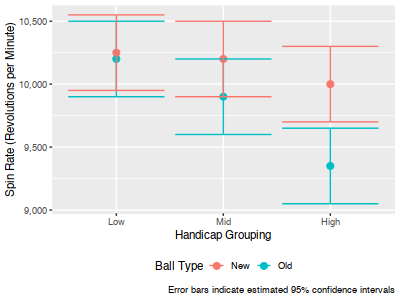
\includegraphics[max width=\linewidth, scale=0.53]{expectations}
    \caption{\label{fig:expectations}Hypothesised relationship between ball type and handicap grouping}
\end{figure}

\end{document}